% This file was created by tikzplotlib v0.9.6.
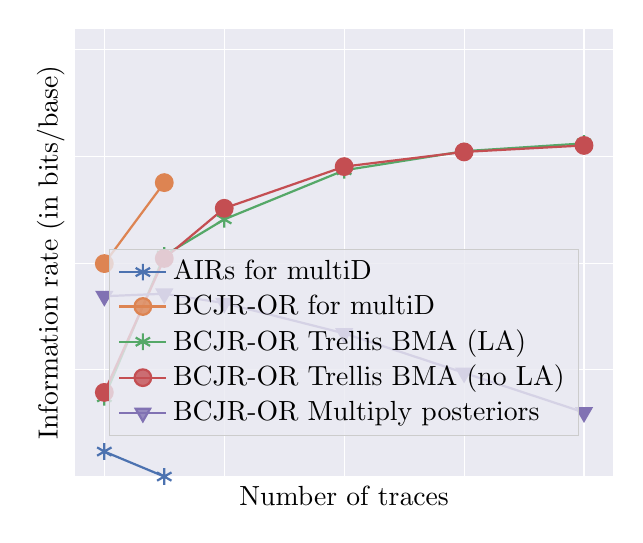
\begin{tikzpicture}

\definecolor{color0}{rgb}{0.917647058823529,0.917647058823529,0.949019607843137}
\definecolor{color1}{rgb}{0.298039215686275,0.447058823529412,0.690196078431373}
\definecolor{color2}{rgb}{0.866666666666667,0.517647058823529,0.32156862745098}
\definecolor{color3}{rgb}{0.333333333333333,0.658823529411765,0.407843137254902}
\definecolor{color4}{rgb}{0.768627450980392,0.305882352941176,0.32156862745098}
\definecolor{color5}{rgb}{0.505882352941176,0.447058823529412,0.701960784313725}

\begin{axis}[
axis background/.style={fill=color0},
axis line style={white},
legend cell align={left},
legend style={fill opacity=0.8, draw opacity=1, text opacity=1, at={(0.5,0.09)}, anchor=south, draw=white!80!black, fill=color0},
tick align=outside,
x grid style={white},
xlabel={Number of traces},
xmajorgrids,
xmajorticks=false,
xmin=1.5, xmax=10.5,
xminorgrids,
xtick style={color=white!15!black},
y grid style={white},
ylabel={Information rate (in bits/base)},
ymajorgrids,
ymajorticks=false,
ymin=0, ymax=2.1,
yminorgrids,
ytick style={color=white!15!black}
]
\addplot [thick, color1, mark=asterisk, mark size=3, mark options={solid}]
table {%
2 0.117128591820664
3 0
};
\addlegendentry{AIRs for multiD}
\addplot [thick, color2, mark=*, mark size=3, mark options={solid}]
table {%
2 0.997606620185793
3 1.37682536480773
};
\addlegendentry{BCJR-OR for multiD}
\addplot [thick, color3, mark=asterisk, mark size=3, mark options={solid}]
table {%
2 0.371059541332272
3 1.03560867847737
4 1.20456448629329
6 1.43449518498082
8 1.52396317364906
10 1.56055426968348
};
\addlegendentry{BCJR-OR Trellis BMA (LA)}
\addplot [thick, color4, mark=*, mark size=3, mark options={solid}]
table {%
2 0.394108232792155
3 1.02166565123491
4 1.25642807834433
6 1.4518180152056
8 1.52063120611686
10 1.55093881644429
};
\addlegendentry{BCJR-OR Trellis BMA (no LA)}
\addplot [thick, color5, mark=triangle*, mark size=3, mark options={solid,rotate=180}]
table {%
2 0.844673581692649
3 0.856268673422246
4 0.812372459591103
6 0.67063732565454
8 0.485817197503681
10 0.300359502207956
};
\addlegendentry{BCJR-OR Multiply posteriors}
\end{axis}

\end{tikzpicture}
